\documentclass[12pt,a4paper]{article}

% ─── Page Layout ───────────────────────────────────────────────────────────────
\usepackage[a4paper, margin=0.8in, headheight=14pt]{geometry}

% ─── Fonts (XeLaTeX) ───────────────────────────────────────────────────────────
\usepackage{fontspec}
\usepackage{unicode-math}
\setmainfont{TeX Gyre Pagella}
\setmonofont[Scale=0.88]{TeX Gyre Cursor}
\setmathfont{Latin Modern Math}

% ─── Packages ──────────────────────────────────────────────────────────────────
\usepackage{xcolor}
\usepackage{colortbl}
\usepackage{titlesec}
\usepackage{enumitem}
\usepackage{tabularx}
\usepackage{booktabs}
\usepackage{array}
\usepackage{amsmath}
\usepackage{tikz}
\usetikzlibrary{shapes.geometric, arrows.meta, positioning, calc, fit, decorations.pathreplacing, decorations.pathmorphing}
\usepackage{tcolorbox}
\tcbuselibrary{skins, breakable}
\usepackage{hyperref}
\usepackage{fancyhdr}
\usepackage{graphicx}
\usepackage{microtype}
\hyphenpenalty=10000
\exhyphenpenalty=10000
\sloppy
\usepackage{caption}
\usepackage{setspace}
\usepackage{multirow}
\usepackage{tocloft}

% ─── Q&A helper ────────────────────────────────────────────────────────────────
\newcommand{\Q}[1]{\textbf{#1}\par\noindent\ignorespaces}

% ─── Colour Palette ────────────────────────────────────────────────────────────
\definecolor{myred}{RGB}{196,30,58}
\definecolor{mydark}{RGB}{30,30,50}
\definecolor{mygreen}{RGB}{14,120,80}
\definecolor{myteal}{RGB}{0,130,140}
\definecolor{myamber}{RGB}{180,100,0}
\definecolor{mypurple}{RGB}{100,30,160}
\definecolor{mygray}{RGB}{246,247,249}
\definecolor{mgframe}{RGB}{180,185,200}
\definecolor{watermark}{RGB}{145,150,170}
\definecolor{hdrred}{RGB}{250,232,235}
\definecolor{hdrgreen}{RGB}{220,244,233}
\definecolor{hdrteal}{RGB}{220,242,244}
\definecolor{hdramber}{RGB}{253,242,215}
\definecolor{hdrpurple}{RGB}{238,228,255}
\definecolor{hdrgray}{RGB}{238,240,245}
\definecolor{rowalt}{RGB}{250,251,253}

% ─── Section Formatting ────────────────────────────────────────────────────────
\titleformat{\section}
  {\large\bfseries\color{myred}}{\thesection.}{0.5em}{}
  [\vspace{1pt}{\color{myred}\rule{\linewidth}{0.8pt}}]
\titleformat{\subsection}
  {\normalsize\bfseries\color{myteal}}{\thesubsection}{0.5em}{}
\titlespacing*{\section}{0pt}{18pt}{7pt}
\titlespacing*{\subsection}{0pt}{11pt}{4pt}

% ─── Paragraph ─────────────────────────────────────────────────────────────────
\setlength{\parindent}{0pt}
\setlength{\parskip}{4pt}

% ─── TOC Styling ───────────────────────────────────────────────────────────────
\renewcommand{\cfttoctitlefont}{\large\bfseries\color{myred}}
\renewcommand{\cftaftertoctitle}{\par\noindent{\color{myred}\rule{\linewidth}{0.8pt}}}
\setlength{\cftbeforetoctitleskip}{0pt}
\setlength{\cftaftertoctitleskip}{6pt}
\renewcommand{\cftsecfont}{\normalsize\bfseries\color{mydark}}
\renewcommand{\cftsecpagefont}{\normalsize\bfseries\color{mydark}}
\renewcommand{\cftsecleader}{\cftdotfill{\cftdotsep}}
\setlength{\cftbeforesecskip}{7pt}
\renewcommand{\cftsubsecfont}{\small\color{mydark}}
\renewcommand{\cftsubsecpagefont}{\small\color{mydark}}
\setlength{\cftbeforesubsecskip}{3pt}
\setlength{\cftsubsecindent}{1.4em}

% ─── Table helpers ─────────────────────────────────────────────────────────────
\renewcommand{\arraystretch}{1.45}
\setlength{\tabcolsep}{6pt}
\arrayrulecolor{mydark}
\newcolumntype{B}[1]{>{\small\bfseries\raggedright\arraybackslash}m{#1}}
\newcolumntype{C}[1]{>{\centering\arraybackslash}m{#1}}
\newcolumntype{Y}{>{\small\raggedright\arraybackslash}X}
\renewcommand{\tabularxcolumn}[1]{m{#1}}

% ─── Header / Footer ───────────────────────────────────────────────────────────
\pagestyle{fancy}
\fancyhf{}
\fancyhead[L]{\small\color{myred}\textbf{PE-EC703C}\;\color{mydark}--- Wavelet Transforms}
\fancyhead[R]{\small\color{myteal}\textbf{Module 6 Notes}}
\fancyfoot[C]{\small\color{mydark}\thepage}
\fancyfoot[R]{\small\color{watermark}\textit{\copyright\ Biraj Sarkar}}
\renewcommand{\headrulewidth}{0.5pt}
\renewcommand{\footrulewidth}{0.3pt}

% ─── Hyperref ──────────────────────────────────────────────────────────────────
\hypersetup{
  colorlinks=true, linkcolor=myteal, urlcolor=myteal,
  pdfauthor={Biraj Sarkar},
  pdftitle={PE-EC703C --- Module 6 Notes}
}

% ─── tcolorbox styles ──────────────────────────────────────────────────────────
\tcbset{
  tikzbox/.style={
    colback=mygray, colframe=mgframe, boxrule=0.6pt, arc=4pt,
    left=8pt, right=8pt, top=6pt, bottom=6pt,
    colbacktitle=mgframe, coltitle=mydark,
    fonttitle=\small\bfseries
  },
  defbox/.style={
    colback=hdrgreen, colframe=mygreen, boxrule=0.8pt, arc=4pt,
    left=9pt, right=9pt, top=6pt, bottom=6pt,
    colbacktitle=mygreen, coltitle=white,
    fonttitle=\small\bfseries
  },
  formulabox/.style={
    colback=hdrteal, colframe=myteal, boxrule=0.8pt, arc=4pt,
    left=9pt, right=9pt, top=7pt, bottom=7pt,
    colbacktitle=myteal, coltitle=white,
    fonttitle=\small\bfseries
  },
  examplebox/.style={
    colback=hdramber, colframe=myamber, boxrule=0.8pt, arc=4pt,
    left=9pt, right=9pt, top=6pt, bottom=6pt,
    colbacktitle=myamber, coltitle=white,
    fonttitle=\small\bfseries
  },
  masonbox/.style={
    colback=hdrpurple, colframe=mypurple, boxrule=0.8pt, arc=4pt,
    left=9pt, right=9pt, top=6pt, bottom=6pt,
    colbacktitle=mypurple, coltitle=white,
    fonttitle=\small\bfseries
  },
  exambox/.style={
    colback=hdrpurple, colframe=mypurple, boxrule=1pt, arc=5pt,
    left=10pt, right=10pt, top=8pt, bottom=8pt,
    colbacktitle=mypurple, coltitle=white,
    fonttitle=\bfseries,
    breakable, title after break={\textbf{Frequently Asked / Viva Questions (contd.)}}}
}
\tcbset{breakable}

% ─── TikZ styles ───────────────────────────────────────────────────────────────
\tikzset{
  block/.style={rectangle, draw=myteal, fill=hdrteal,
    text width=2.4cm, align=center, minimum height=0.95cm,
    font=\small, rounded corners=3pt, line width=0.7pt},
  redblock/.style={rectangle, draw=myred, fill=hdrred,
    text width=2.4cm, align=center, minimum height=0.95cm,
    font=\small, rounded corners=3pt, line width=0.7pt},
  arrow/.style={-Stealth, thick, color=mydark},
  redarrow/.style={-Stealth, thick, color=myred},
  line/.style={thick, color=mydark}
}

% ═══════════════════════════════════════════════════════════════════════════════
\begin{document}
% ═══════════════════════════════════════════════════════════════════════════════

\begin{center}
  {\LARGE\bfseries\color{myred} PE-EC703C --- Wavelet Transforms}\\[5pt]
  {\normalsize\color{mydark} Semester VII \quad$\bullet$\quad 3L:0T:0P \quad$\bullet$\quad 3 Credits}\\[3pt]
  {\normalsize\color{myteal}\textbf{Module 6 Exam Notes: Wavelet Transform and Applications}}\\[3pt]
  {\small\color{mydark} CGEC \;$|$\; B.Tech ECE (2023--27) \;$|$\; \textit{Biraj Sarkar}}
\end{center}
\noindent{\color{myred}\rule{\linewidth}{1.5pt}}
\vspace{2pt}

\hypersetup{linkcolor=mydark}
\tableofcontents
\hypersetup{linkcolor=myteal}
\newpage

% ===============================================================================
\section{Transform Coding and Data Compression}
% ===============================================================================

Data compression reduces transmission bandwidth and storage requirements. In \textbf{Transform Coding}, a mathematical transform maps spatial/temporal domain signal values to a frequency-like domain, where the coefficients are less correlated and easier to compress.

\subsection{Principles of Transform Coding}
Transform coding relies on three core steps:
\begin{enumerate}[leftmargin=*, itemsep=4pt]
  \item \textbf{Transform:} De-correlates the signal data, packing most of the energy into a few high-magnitude coefficients (Energy Compaction).
  \item \textbf{Quantization:} Converts continuous or high-precision coefficients to discrete levels. This is a lossy step where small, high-frequency coefficients (representing details less perceptible to human eyes/ears) are rounded to zero.
  \item \textbf{Entropy Coding:} Applies lossless compression (e.g., Huffman or Arithmetic coding) to the quantized symbols, mapping more frequent values to shorter codewords.
\end{enumerate}

\subsection{Image and Audio Compression: DWT/DTWT vs. DCT (JPEG 2000 vs. JPEG)}
For discrete-time sequences (such as digital audio and images), the Discrete Wavelet Transform is implemented as the \textbf{Discrete-Time Wavelet Transform (DTWT)} using digital filter banks.
\begin{itemize}[leftmargin=*, itemsep=4pt]
  \item \textbf{JPEG (Discrete Cosine Transform):} Splits an image into non-overlapping $8 \times 8$ blocks and applies 2D DCT to each block. At high compression ratios, discarding high-frequency coefficients creates artificial grid-like discontinuities at block boundaries, known as \textbf{blocking artifacts}.
  \item \textbf{JPEG 2000 (Discrete Wavelet Transform):} Applies DWT globally over the entire image (or large tile regions). This eliminates blocking artifacts, resulting in graceful, blurry degradation rather than grid patterns. 
  \item \textbf{Key Advantages of JPEG 2000 over JPEG:}
        \begin{itemize}[leftmargin=*, itemsep=2.5pt, topsep=2pt]
          \item \textbf{No Blocking Artifacts:} Smooth, visually superior reconstruction at low bitrates.
          \item \textbf{Progressive Transmission:} Single bitstream contains multiple resolutions and quality layers. A low-resolution thumbnail is decoded first, followed by details as more data arrives.
          \item \textbf{Region of Interest (ROI) Coding:} Particular regions of an image (e.g., a tumor in a medical scan) can be encoded with higher precision than the background.
          \item \textbf{Unified Lossless and Lossy:} Uses the CDF 5/3 filter bank for lossless compression and the CDF 9/7 filter bank for lossy compression.
        \end{itemize}
\end{itemize}

\par\noindent
{\renewcommand{\arraystretch}{1.4}%
\begin{tabularx}{\linewidth}{|B{3.5cm}|Y|Y|}
\hline
\textbf{Feature} & \textbf{Standard JPEG (DCT-based)} & \textbf{JPEG 2000 (DWT-based)} \\
\hline
\textbf{Core Transform} & Block-based Discrete Cosine Transform (DCT). & Discrete Wavelet Transform (DWT). \\
\hline
\textbf{Processing Unit} & Fixed $8 \times 8$ pixel blocks. & Entire image or large tile regions. \\
\hline
\textbf{Compression Ratio} & Poor quality at ratios $> 30:1$ (blocks visible). & Excellent quality at high ratios ($> 100:1$). \\
\hline
\textbf{Artifact Type} & Blocking artifacts (grid patterns) and mosquito noise. & Blurring and ringing artifacts around edges. \\
\hline
\textbf{Scalability} & Not natively supported (needs separate files). & Resolution and quality scalability in one stream. \\
\hline
\textbf{Entropy Coder} & Huffman Coding. & Context-adaptive EBCOT (Arithmetic Coding). \\
\hline
\end{tabularx}}

\subsection{Audio Coding and Video Coding}
\begin{itemize}[leftmargin=*, itemsep=4pt]
  \item \textbf{Audio Coding:} The human ear acts as a spectrum analyzer. Wavelet-based audio coders exploit this multi-resolution structure. By dividing the audio spectrum into subbands matching the ear's \textbf{critical bands}, subband coding allocates bits dynamically based on psychoacoustic masking (louder sounds mask quieter adjacent frequencies).
  \item \textbf{Video Coding:} Standard video codecs (H.264/H.265) utilize block-based motion estimation and DCT. Wavelet-based video coding uses DWT on individual frames or applies a \textbf{3D DWT} (spatial $x$-$y$ DWT + temporal $t$ DWT) to compress spatial and motion information simultaneously, avoiding motion compensation loops.
\end{itemize}

% ===============================================================================
\section{Wavelet De-noising and Image Processing}
% ===============================================================================

\subsection{Wavelet De-noising (Hard vs. Soft Thresholding)}
Consider a noisy signal model:
$$y_i = x_i + \sigma z_i, \quad i = 1, 2, \dots, N$$
where $y_i$ is the observed noisy signal, $x_i$ is the clean signal, $\sigma$ is the noise standard deviation, and $z_i \sim \mathcal{N}(0, 1)$ is additive white Gaussian noise (AWGN).

Since DWT is a linear orthogonal transform, the noise remains white and spread evenly across all coefficients, whereas the signal energy is concentrated into a few large wavelet coefficients. Denoising is achieved by thresholding the DWT coefficients.

\begin{tcolorbox}[formulabox, title={\textbf{Hard and Soft Thresholding Formulations}}]
Let $w$ represent a wavelet coefficient, and $\lambda$ be the threshold limit ($\lambda > 0$).
\begin{enumerate}[leftmargin=*, itemsep=4pt, label=\arabic*.]
  \item \textbf{Hard Thresholding:} Sets coefficients below the threshold to zero, keeping the others unchanged:
        $$\eta_\lambda^{\text{hard}}(w) = \begin{cases} w, & |w| > \lambda \\ 0, & |w| \le \lambda \end{cases}$$
  \item \textbf{Soft Thresholding (Wavelet Shrinkage):} Sets coefficients below the threshold to zero, and shrinks the remaining coefficients towards zero:
        $$\eta_\lambda^{\text{soft}}(w) = \text{sgn}(w)\max(|w| - \lambda, 0)$$
\end{enumerate}
\tcbset{after={\color{black}}}
\end{tcolorbox}

\begin{itemize}[leftmargin=*, itemsep=4.5pt]
  \item \textbf{Comparison:} Hard thresholding preserves edge sharpness but can introduce spurious oscillations (pseudo-Gibbs phenomena) due to the discontinuity in the thresholding function. Soft thresholding is continuous, yielding smoother denoised signals, but it introduces a bias by scaling down large coefficients, which slightly blurs sharp peaks.
\end{itemize}

\subsection{Threshold Selection Rules}
\begin{itemize}[leftmargin=*, itemsep=4.5pt]
  \item \textbf{VisuShrink (Universal Threshold):} Uses a global threshold derived by Donoho and Johnstone:
        $$\lambda_{\text{univ}} = \sigma \sqrt{2 \ln N}$$
        where $N$ is the length of the signal. It guarantees with high probability that the maximum noise coefficient is below $\lambda$. However, for large $N$, $\lambda_{\text{univ}}$ becomes large, causing over-smoothing (loss of fine details). The noise variance $\sigma$ is estimated from the median absolute deviation (MAD) of the finest detail subband ($HH_1$):
        $$\hat{\sigma} = \frac{\text{median}(|w_{j,k}|)}{0.6745}, \quad w_{j,k} \in \text{finest subband}$$
  \item \textbf{SureShrink:} An adaptive, subband-dependent thresholding method. For each subband, it selects a threshold $\lambda$ that minimizes \textbf{Stein's Unbiased Risk Estimate (SURE)}, optimizing the mean squared error (MSE) estimate.
\end{itemize}

\begin{tcolorbox}[tikzbox, title={Wavelet-Based Denoising Process Flow}]
\centering
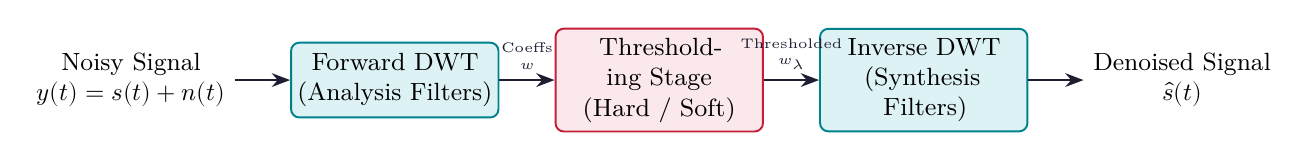
\begin{tikzpicture}[node distance=1.0cm and 0.8cm, auto]
  \node (input) [align=center, font=\small] {Noisy Signal\\$y(t) = s(t) + n(t)$};
  \node (dwt) [block, right=0.7cm of input] {Forward DWT\\(Analysis Filters)};
  \node (thresh) [redblock, right=0.7cm of dwt] {Thresholding Stage\\(Hard / Soft)};
  \node (idwt) [block, right=0.7cm of thresh] {Inverse DWT\\(Synthesis Filters)};
  \node (output) [right=0.7cm of idwt, align=center, font=\small] {Denoised Signal\\$\hat{s}(t)$};

  \draw [arrow] (input) -- (dwt);
  \draw [arrow] (dwt) -- node[above, font=\tiny, align=center] {Coeffs\\$w$} (thresh);
  \draw [arrow] (thresh) -- node[above, font=\tiny, align=center] {Thresholded\\$w_\lambda$} (idwt);
  \draw [arrow] (idwt) -- (output);
\end{tikzpicture}
\end{tcolorbox}

\subsection{Speckle Removal (Homomorphic Wavelet Filtering)}
Speckle is a high-frequency multiplicative noise common in coherent imaging systems like Synthetic Aperture Radar (SAR) and Ultrasound:
$$y = x \cdot n$$
where $y$ is the observed image, $x$ is the noise-free image, and $n$ is the speckle noise.
Standard denoising assumes additive noise. To resolve this, \textbf{Homomorphic Filtering} is applied:
\begin{enumerate}[leftmargin=*, itemsep=4pt]
  \item Take the logarithm of the noisy image to convert multiplicative noise into additive noise:
        $$\ln(y) = \ln(x) + \ln(n) \implies y' = x' + n'$$
  \item Apply DWT to $y'$, perform thresholding on the detail subbands, and apply IDWT to get the denoised estimate $\hat{x}'$.
  \item Exponentiate the result to return to the original scale:
        $$\hat{x} = \exp(\hat{x}')$$
\end{enumerate}

\subsection{Edge Detection and Object Isolation}
\begin{itemize}[leftmargin=*, itemsep=4.5pt]
  \item \textbf{Edge Detection:} Sharp changes in image intensity (edges) correspond to local maxima of the wavelet transform modulus at fine scales. By observing coefficients across multiple scales, we can distinguish true edges (which persist across scales) from random noise (which rapidly decays at coarser scales).
  \item \textbf{Image Fusion:} Combines complementary information from multiple images of the same scene (e.g., multi-focus or infrared/visible cameras). The source images are decomposed using DWT. The coefficient subbands are fused:
        \begin{itemize}[leftmargin=*, itemsep=2.5pt, topsep=2pt]
          \item \textbf{LL (Approximation) Coefficients:} Typically averaged to preserve average illumination.
          \item \textbf{Detail Coefficients (LH, HL, HH):} Selected using a "maximum absolute value" rule, as larger coefficients correspond to sharper, in-focus features.
        \end{itemize}
        Applying the IDWT to the fused coefficients yields a single high-quality composite image.
\end{itemize}

% ===============================================================================
\section{Discrete Wavelet Multi-Tone Modulation (DWMT)}
% ===============================================================================

\begin{tcolorbox}[defbox, title={\textbf{Definition of DWMT}}]
\textbf{Discrete Wavelet Multi-Tone (DWMT)} modulation is a multicarrier communication technique that uses Orthogonal Wavelet Filter Banks (specifically, Cosine-Modulated Filter Banks or Synthesis/Analysis Wavelet filters) as subcarrier generators instead of the DFT/IDFT used in standard OFDM.
\end{tcolorbox}

In standard \textbf{OFDM (Orthogonal Frequency Division Multiplexing)}, subcarriers are shaped like sinc functions because they are modulated by a rectangular window. This yields high spectral sidelobes ($-13\text{ dB}$). Any frequency offset causes \textbf{Inter-Carrier Interference (ICI)}, requiring a \textbf{Cyclic Prefix (CP)} guard interval which reduces spectral efficiency by $10\text{--}25\%$.

\subsubsection{Advantages of DWMT over OFDM:}
\begin{enumerate}[leftmargin=*, itemsep=4pt]
  \item \textbf{Low Sidelobes:} Wavelet filters have excellent spectral containment, with sidelobes decaying much faster than $-13\text{ dB}$ (often below $-40\text{ dB}$).
  \item \textbf{No Cyclic Prefix:} Because spectral overlap between non-adjacent subcarriers is negligible, DWMT does not require a cyclic prefix. This saves transmission bandwidth.
  \item \textbf{High ICI/ISI Immunity:} The high stop-band attenuation of wavelet filters makes DWMT robust against narrowband interference and multipath channel distortions.
\end{enumerate}

\newpage
% ===============================================================================
\begin{center}
  {\large\bfseries\color{myred} Quick Revision --- Module 6}\\[3pt]
  {\small\color{mydark} Wavelet Transform and Applications $|$ PE-EC703C}
\end{center}
\noindent{\color{myred}\rule{\linewidth}{1.2pt}}
\vspace{4pt}
% ===============================================================================

\begin{tcolorbox}[formulabox, title={\textbf{Key Equations}}]
\renewcommand{\arraystretch}{1.35}
\begin{tabularx}{\linewidth}{B{5.0cm} X}
Hard Thresholding & $\eta_\lambda^{\text{hard}}(w) = \begin{cases} w, & |w| > \lambda \\ 0, & |w| \le \lambda \end{cases}$ \\[12pt]
Soft Thresholding & $\eta_\lambda^{\text{soft}}(w) = \text{sgn}(w)\max(|w| - \lambda, 0)$ \\[4pt]
Universal Threshold & $\lambda_{\text{univ}} = \sigma \sqrt{2 \ln N}$ \\[4pt]
Noise Variance Estimate & $\hat{\sigma} = \frac{\text{median}(|w_{j,k}|)}{0.6745} \quad (w_{j,k} \in \text{finest subband } HH_1)$
\end{tabularx}
\tcbset{after={\color{black}}}
\end{tcolorbox}

\begin{tcolorbox}[defbox, title={\textbf{One-Line Definitions}}]
\begin{itemize}[leftmargin=*, itemsep=3.5pt]
  \item \textbf{Energy Compaction:} Concentrate signal representation into a small number of large coefficients.
  \item \textbf{Blocking Artifacts:} Grid-like boundaries visible at low bitrates in block-based DCT compression.
  \item \textbf{Wavelet Shrinkage:} Noise reduction method that attenuates coefficients toward zero (soft thresholding).
  \item \textbf{VisuShrink:} Denoising method using the universal threshold $\sigma \sqrt{2 \ln N}$ to remove noise with high probability.
  \item \textbf{SureShrink:} Adaptive denoising scheme minimizing Stein's Unbiased Risk Estimate for each subband.
  \item \textbf{Homomorphic Filter:} Transform mapping multiplicative noise to additive noise via log operations.
  \item \textbf{DWMT Modulation:} Multicarrier modulation using wavelet synthesis/analysis filter banks instead of DFT.
\end{itemize}
\end{tcolorbox}

\begin{tcolorbox}[exambox, title={\textbf{Frequently Asked / Viva Questions}}]
\begin{enumerate}[topsep=0pt, label=\textbf{Q\arabic*.}, itemsep=5pt]
  \item \Q{Why does JPEG 2000 perform better than standard JPEG at low bitrates?}
        Standard JPEG uses block-based DCT ($8 \times 8$), which causes blocking artifacts due to independent processing of boundaries. JPEG 2000 uses DWT globally on the entire image, which yields no block borders and results in a graceful blur at low bitrates.

  \item \Q{Compare hard and soft thresholding in terms of visual quality and math.}
        Hard thresholding is discontinuous and keeps coefficients larger than $\lambda$ unchanged, which preserves sharp edges but can create pseudo-Gibbs oscillations. Soft thresholding is continuous and reduces coefficients by $\lambda$, which yields smoother signals but introduces bias and blurs sharp peaks.

  \item \Q{What is the universal threshold in VisuShrink, and what is its drawback?}
        $\lambda_{\text{univ}} = \sigma \sqrt{2 \ln N}$. Its drawback is that as signal length $N$ increases, the threshold becomes excessively large. This removes almost all noise but also removes true high-frequency signal details, causing over-smoothing.

  \item \Q{How do we estimate the noise variance $\sigma$ in practical image denoising?}
        It is estimated from the median absolute deviation (MAD) of the finest detail subband coefficients ($HH_1$): $\hat{\sigma} = \text{median}(|w_{j,k}|) / 0.6745$.

  \item \Q{Explain the homomorphic wavelet denoising workflow for speckle noise.}
        Speckle is multiplicative ($y = x \cdot n$). We apply a logarithmic transform: $\ln(y) = \ln(x) + \ln(n)$ to convert it to additive noise. We then apply DWT, perform wavelet thresholding, apply IDWT, and finally exponentiate the result.

  \item \Q{How is DWT used for image fusion?}
        Multiple source images are decomposed by DWT. The LL (approximation) coefficients are averaged to preserve illumination, and the detail coefficients (LH, HL, HH) are fused by taking the maximum absolute value (which preserves sharp details and focus). The fused image is reconstructed using IDWT.

  \item \Q{What are the advantages of DWMT over OFDM?}
        DWMT uses wavelet filter banks which have much lower sidelobes than OFDM's sinc subcarriers. This reduces Inter-Carrier Interference (ICI) and eliminates the need for a Cyclic Prefix (CP), increasing spectral efficiency.
\end{enumerate}
\end{tcolorbox}

\begin{tcolorbox}[tikzbox, title={\textbf{JPEG vs. JPEG 2000 Comparison Matrix}}]
\par\noindent
{\renewcommand{\arraystretch}{1.4}%
\begin{tabularx}{\linewidth}{|B{3.2cm}|Y|Y|}
\hline
\textbf{Feature} & \textbf{Standard JPEG (DCT-based)} & \textbf{JPEG 2000 (DWT-based)} \\
\hline
\textbf{Core Transform} & Block-based Discrete Cosine Transform (DCT). & Discrete Wavelet Transform (DWT). \\
\hline
\textbf{Processing Unit} & Fixed $8 \times 8$ pixel blocks. & Entire image or large tile regions. \\
\hline
\textbf{Compression Ratio} & Poor quality at ratios $> 30:1$ (blocks visible). & Excellent quality at high ratios ($> 100:1$). \\
\hline
\textbf{Artifact Type} & Blocking artifacts (grid patterns) and mosquito noise. & Blurring and ringing artifacts around edges. \\
\hline
\textbf{Scalability} & Not natively supported (needs separate files). & Resolution and quality scalability in one stream. \\
\hline
\textbf{Entropy Coder} & Huffman Coding. & Context-adaptive EBCOT (Arithmetic Coding). \\
\hline
\end{tabularx}}
\end{tcolorbox}

\end{document}
